\begin{frame}{L'utopie de la désintermédiation}
    Selon Marin Dacos et Pierre Mounier dans \textit{L'édition en réseau}:\\
    "la fonction du médiateur qu'est l'éditeur n'a pas disparu" mais simplement "profondément changé et contraint tous les acteurs traditionnels à redéfinir d'urgence les bases de leur métier sous peine de disparaître au profit d'acteurs nouveaux venant d'autres horizons."\\
    \vspace{1em}
    \textrightarrow{} Remplacement de ses anciens intermédiaires par de nouveaux acteurs.
\end{frame}

\begin{frame}{L'utopie de la désintermédiation}
    \begin{columns}
    % Colonne de gauche : Texte
        \begin{column}{0.5\textwidth}
            \small
                \textit{La situation de ces marchés peut ainsi être qualifiée d'oligopole à franges, c'est à dire un marché structuré principalement autour d'un nombre réduit d'acteurs captant la majeure partie du marché et entourés d'un grand nombre d'acteurs de taille bien plus réduite se partageant une part très limitée du marché. Cette tectonique des usages numériques a abouti à l'émergence d'acteurs largement dominants regoupés sous l'acronyme GAFAM pour Google, Apple, Facebook, Amazon et Microsoft.}\\
\textbf{L’édition à l’époque du numérique, Benoît Epron et Marcello Vitali-Rosati, 2018.}
        \end{column}

        % Colonne de droite : Image
        \begin{column}{0.4\textwidth}
            \centering
            
\includegraphics[width=\textwidth]{images/DRE351OXkAAJHxU.jpg}
        \end{column}
    \end{columns}
\end{frame}
\begin{frame}{De la désintermédiation à la réintermédiation}
    Selon Vincent Bullich dans \textit{La « plateformisation » comme déploiement d’une logique organisatrice : propositions théoriques et éléments de méthode}:\\
    \begin{itemize}
        \item La désintermédiation devait reconfigurer les économies et les modalités de communication en favorisant une "immédiateté entre offre et demande".
        \item MAIS inverse: multiplication des acteurs autour des plateformes.
    \end{itemize}
    \vspace{1em}
\begin{figure}
    \centering
    
\includegraphics[width=.55\textwidth]{images/kindle_plateforme.png}
\end{figure}
\end{frame}

\begin{frame}{De la désintermédiation à la réintermédiation}
    \begin{columns}
    % Colonne de gauche : Texte
        \begin{column}{0.45\textwidth}
            \begin{itemize}
                \item Depuis juillet 2015, les auteur.rices dont les livres sont empruntés via plateforme ne sont plus rémunéré.es selon le barème d’une base minimale de lecture de 10\% du livre, mais en fonction du nombre de pages lues.
                \item Formatage des écrits pour inciter, coûte que coûte, le lecteur à poursuivre le plus loin possible sa progression dans l’ouvrage ?
            \end{itemize}
        \end{column}

        % Colonne de droite : Image
        \begin{column}{0.5\textwidth}
            \centering
            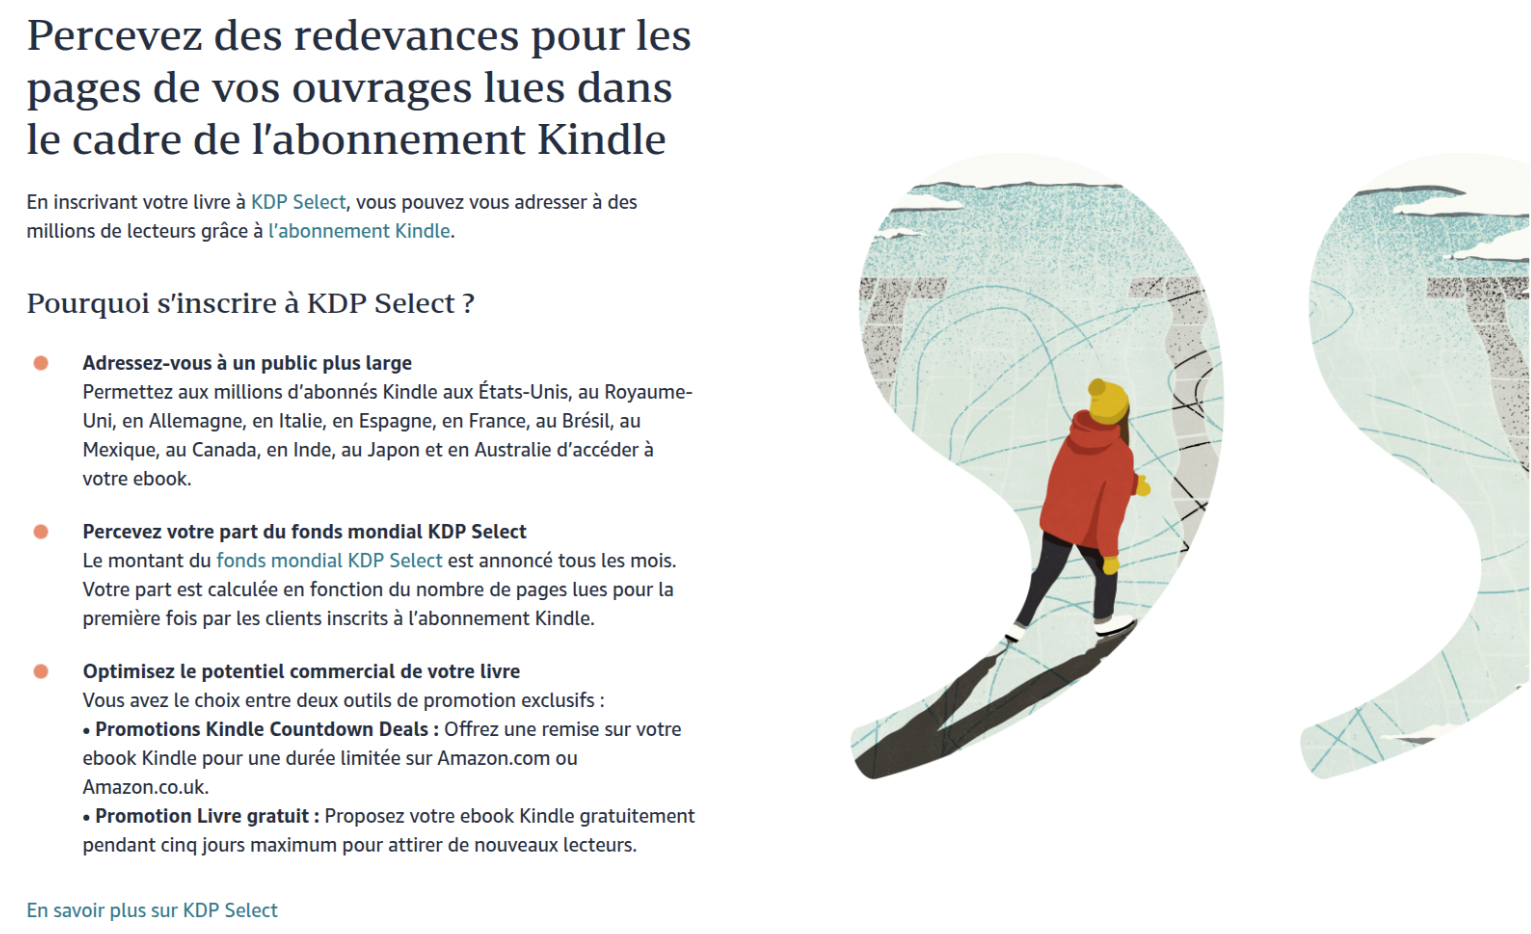
\includegraphics[width=\textwidth]{images/kindle_plateforme2.png}
        \end{column}
    \end{columns}
\end{frame}

\begin{frame}{De la désintermédiation à la réintermédiation}
    \begin{columns}
    % Colonne de gauche : Texte
        \begin{column}{0.4\textwidth}
            \begin{itemize}
                \item \textit{Amazon, par exemple, ne se contente pas de savoir quels livres ses clients achètent sur sa plateforme, il analyse aussi les traces de la vitesse de lecture sur la liseuse : lire le livre en entier ou non, sauter des chapitres, etc.} \textbf{[Dominique Cardon, Culture numérique, 2019]}
            \end{itemize}
        \end{column}

        % Colonne de droite : Image
        \begin{column}{0.5\textwidth}
            \centering
            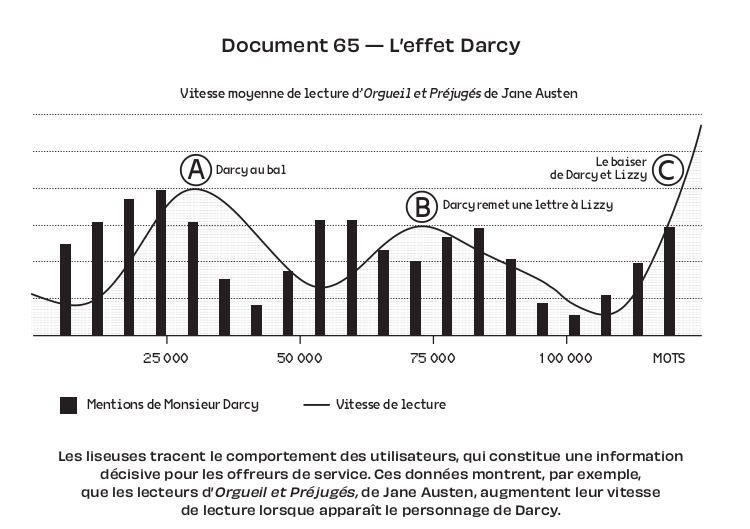
\includegraphics[width=\textwidth]{images/effetDarcy.png}
        \end{column}
    \end{columns}
\end{frame}

\begin{frame}{Réintermédiation numérique : le risque de la plateformisation}
    \textbf{Plateforme = } Logiciels construits par des sociétés à des fins commerciales.\\
    \vspace{1em}
    
    Mounier et Dacos parlent de facteurs de réintermédiation via : 
    \begin{itemize}
        \item le design des plateformes informatiques ;
        \item la définition des règles d'écriture et de lecture ;
        \item la gestion des communautés qui les utilisent ;
        \item les algorithmes de classement de l'information produite.
    \end{itemize}
    \textbf{Plateformisation =} Uniformisation des productions dans un format de publication préconstruit et partagé par une communauté d'utilisateur.rices, avec les dérives potentielles en termes de censure, formatage, appauvrissement de contenu etc...\\
\end{frame}